\documentclass[11pt,a4paper,twoside]{article}

%\usepackage{algorithm}  
%\usepackage{algorithmic}  

\usepackage{CJK}
\usepackage[utf8]{inputenc}
\usepackage{amsmath}
\usepackage{amsthm}

%图片标题是多行也能保持居中
\usepackage[centerlast]{caption}

\usepackage{amsfonts}
\usepackage{amssymb}
\usepackage{graphicx}
\counterwithin{figure}{section}
%\usepackage{fourier}
\usepackage[left=2cm,right=2cm,top=2cm,bottom=2cm]{geometry}

%定义作者的包
\usepackage{authblk}
%删除线的包
\usepackage{ulem}

%设置缩进
\usepackage{indentfirst} 
\setlength{\parindent}{2em}

%设置行距
\linespread{1.2}

%c++代码显示环境
\usepackage{listings}
\lstset{language=MATLAB}

%算法伪代码环境
\usepackage[ruled,vlined]{algorithm2e}
%\usepackage[linesnumbered,lined,boxed,commentsnumbered]{algorithm2e}
%\usepackage{algorithm}
%\usepackage{algorithmic}


\title{A Singularly Valuable Decomposition: The SVD
of a Matrix\\
奇异值分解:矩阵的SVD
}
\author{Dan Kalman\\
The American University\\
Washington, DC 20016}
\date{February 13, 2002}

\begin{document}

\begin{CJK}{UTF8}{gbsn}
\maketitle

\begin{abstract}
每一位线性代数老师都应该熟悉矩阵奇异值分解(或SVD)。它具有有趣和吸引人的代数性质,并传达了关于线性变换的重要几何和理论见解。SVD和对称矩阵对角化理论之间的紧密联系使得线性代数老师们可以立即接触到这个话题,事实上,这是这些老师已经知道的内容的自然延伸。同时,奇异值分解在线性代数的几种不同应用中具有重要的基础意义。当斯特朗在他现在的经典著作[22,142页]中介绍SVD时,他就意识到了这些事实

\textbf{.. 它远没有它应有的名气。}

Golub和Van Loan在他们对数值矩阵方法的明确解释中认为SVD具有中心意义[8,第xiv页]

\textbf{...也许这本书中最反复出现的主题是[$S V D]$的实践和理论价值}

SVD的重要性的其他证据是它在近年来《数学杂志》和《美国数学月刊》上的许多论文中的核心作用(例如$[2,3,17,23]$)。

虽然把SVD包括在第一门线性代数课程中可能是不可行的,但它绝对值得在更高级的本科课程中占有一席之地,特别是那些侧重于数字或应用的课程。我在这篇文章中的主要目标是让广大读者注意到这个话题,并揭示一些给予它实践和理论意义的方面。
\end{abstract}


\section{理论}
SVD与我们熟悉的对称矩阵对角化理论密切相关。回想一下,如果$A$是一个对称的实$n \times n$矩阵,则存在一个正交矩阵$V$和一个对角矩阵$D$使$A=V D V^{T}$。这里$V$的列是$A$的特征向量,并形成$\mathbf{R}^{\mathbf{n}}$的标准正交基;$D$的对角线项是$A$的特征值。为了强调与SVD的联系,我们称$V D V^{T}$为特征值分解,或$A$的$EVD $。

对于SVD,我们从一个任意的实际$m \times n$矩阵$A$开始。正如我们将看到的,有正交矩阵$U$和$V$和一个对角矩阵,这次表示为$\Sigma$,这样$ A =U \Sigma V^{T}$。在这种情况下,$U$是$m \times m$, $V$是$n \times n$,因此$\Sigma$是矩形,与$A$具有相同的尺寸。$\Sigma$的对角线项,即$\Sigma_{i i}=\sigma_{i}$,可以按大小递减的顺序排列为非负的。正的称为$A$的奇异值。$U$和$V$的列分别称为$A$的左奇异向量和右奇异向量。

通过将矩阵看作线性变换,对称矩阵的EVD和任意矩阵的SVD之间的相似性可以得到扩展。对于对称矩阵$ A $,变换取$\mathbf{R}^{\mathbf{n}}$为自身,而$V$的列定义了一个特别好的基。当向量相对于这个基表示时,我们可以看到,根据特征值的大小,这个变换简单地将一些分量展开,并将另一些分量收缩(对于负的特征值,通过原点的反射)。而且,这个基是正交的,这是最好的一种基。


现在让我们看看一个$m \times n$矩阵$A$的SVD。在这里,转换需要$\mathbf{R}^{\mathbf{n}}$到不同的空间,$\mathbf{R}^{\mathbf{m}}$,所以合理的是要求每个域和范围的自然基。$V$和$U$列提供了这些基础。当它们被用来表示变换的域和范围内的向量时,变换的性质再次变得透明:它根据奇异值的大小,简单地扩大一些分量,收缩其他分量,并可能丢弃分量或根据需要添加零来解释维数的变化。从这个角度来看,SVD告诉我们如何选择标准正交基,以便用最简单的矩阵(即对角线)表示变换。

我们如何选择基 $\left\{v_{1}, v_{2}, \cdots, v_{n}\right\}$ 和 $\left\{u_{1}, u_{2}, \ cdots, u_{m}\right\}$ 用于域和范围?获得对角线表示并不困难。为此,我们只需要 $A v_{i}=\sigma_{i} u_{i}$,这很容易处理。为 $\mathbf{R}^{\mathbf{n}}$ 选择一个正交基 $\left\{v_{1}, v_{2}, \cdots, v_{n}\right\}$ 使得前 $k$ 元素跨越 $A$ 的行空间,其余 $n-k$ 元素跨越 $A$ 的空空间,其中 $k$ 是 $A$ 的rank()。然后对于 $1 \leq i \leq k$ 定义 $u_{i}$ 为平行于 $A v_{i}$ 的单位向量,并将其扩展为 $\mathbf{R}^{\mathbf{ m}}$。相对于这些底,$A$ 将具有对角线表示。但总的来说,尽管 $v$ 是正交的,但没有理由期望 $u$ 是正交的。选择 $v$-basis 以使其正交性保持在 $A$ 下的可能性是关键点。接下来我们展示$n \times n$ 对称矩阵$A^{T} A$ 的EVD 提供了这样一个基础,即$A^{T} A$ 的特征向量。

设$A^{T} A=V D V^{T}$, $D$的对角线项$\lambda_{i}$按非递增的顺序排列,并设$V$的列($A^{T} A$的特征向量)是标准正交基$\left\{v_{1},v_{2}, \cdots, v_{n}\right\}$。然后
$$
A v_{i} \cdot A v_{j}=\left(A v_{i}\right)^{T}\left(A v_{j}\right)=v_{i}^{T} A^{T} A v_{j}=v_{i}^{T}\left(\lambda_{j} v_{j}\right)=\lambda_{j} v_{i} \cdot v_{j}
$$
所以图像集$\left\{A v_{1}, A v_{2}, \cdots, A v_{n}\right\}$是正交的,并且这个集合中的非零向量形成了$A$范围的一组基。因此,$A^{T} A$及其在$A$下的图像的特征向量提供了正交基,使得$A$可以用对角线的形式表示。

为了完成构造,我们将向量$A v_{i}$归一化。在这一步中,$A^{T} A$的特征值再次出现。在上面的计算中,$i=j$给出$\left|A v_{i}\right|^{2}=\lambda_{i}$,这意味着$\lambda_{i} \geq 0$。由于假设这些特征值以非递增的顺序排列,我们得出$\lambda_{1} \geq \lambda_{2} \geq \cdots \geq \lambda_{k} \geq$ 0和,由于$A$的秩等于$k$, 当$i>k$时 $\lambda_{i}=0$ 。因此,值域的标准正交基由
$$
u_{i}=\frac{A v_{i}}{\left|A v_{i}\right|}=\frac{1}{\sqrt{\lambda_{i}}} A v_{i} ; \quad 1 \leq i \leq k
$$
如果 $k<m$,我们将其扩展到 $\mathbf{R}^{\mathbf{m}}$ 的正交基。

这样就完成了 $\mathbf{R}^{\mathbf{n}}$ 和 $\mathbf{R}^\mathbf{m}$ 的所需正交基的构造。 设置 $\sigma_{i}=\sqrt{\lambda_{i}}$ 我们有 $A v_{i}=\sigma_{i} u_{i}$ 对于所有 $i \leq k$。 将$v_{i}$ 组装成矩阵$V$ 和$u_{i}$ 的列组成$U$,这表明$A V=U \Sigma$,其中$\Sigma$ 具有相同的 维度为 $A$,沿主对角线具有元素 $\sigma_{i}$,并且所有其他元素均为零。 因此,$A=U \Sigma V^{T}$,即$A$的奇异值分解。

综上所述,$m \times n$ 实矩阵 $A$ 可以表示为乘积 $U \Sigma V^{T}$,其中 $V$ 和 $U$ 是正交矩阵,$\Sigma$ 是 对角矩阵,如下。 矩阵$V$由对角分解$A^{T} A=V D V^{T}$得到,其中$D$的对角元素以非递增顺序出现; $U$ 的列来自于对 $V$ 列的 $A$ 下的非消失图像进行归一化,并扩展(如果需要)到 $\mathbf{R}^{\mathbf{m}}$ 的正交基 ; $\Sigma$ 的非零条目是 $D$ 的对应对角线条目的相应平方根。

前面的构造证明了 SVD 的存在,并给出了一些关于它所讲述的矩阵的概念。 还有许多关于 SVD 的额外代数和几何见解,这些见解同样容易推导出来。 在进行这些见解之前,应该做两点评论。 首先,SVD 封装了矩阵 $A$ 定义的线性变换的域和范围的最合适的基。 这些基础和与 $A$ 相关的四个基本子空间之间存在着一种美妙的关系:范围和零空间,以及它们的正交补码。 正是 SVD 和这些子空间提供的全貌,Strang 称之为线性代数的基本定理。 他还发明了一个示意图,示意性地说明了基数和四个子空间的关系(见图(\ref{fig:1}))。 推荐 Strang 的文章 [23] 详细讨论该主题。

第二个标记涉及计算。数学理论和计算实践之间经常存在差距。理论上,我们设想以无限精度对实数进行算术运算。但是当我们在数字计算机上进行算术运算时,我们不是用实数计算,而是用一组有限的有理数计算,结果只能以有限的精度逼近真实的计算。理论上看起来优雅而直接的程序有时作为计算算法的处方可能存在严重缺陷。 SVD 说明了这一点。我们的构造似乎为 SVD 提供了一种简单的算法:形成 $A^{T} A$,计算其特征值和特征向量,然后如上所述找到 SVD。在这里,实践和理论分道扬镳。正如我们稍后将看到的,$A^{T}A$ 的计算可能会严重损失精度。事实证明,在不形成 $A^{T} A$ 的情况下找到 $A$ 的 SVD 的直接方法是存在的,事实上,在许多应用中,SVD 的实际重要性在于它允许人们找到 $A^{T} A$ 的 EVD,而无需形成这种数值上的危险乘积。

\begin{figure}[htbp]%[htbp]
  \centering
  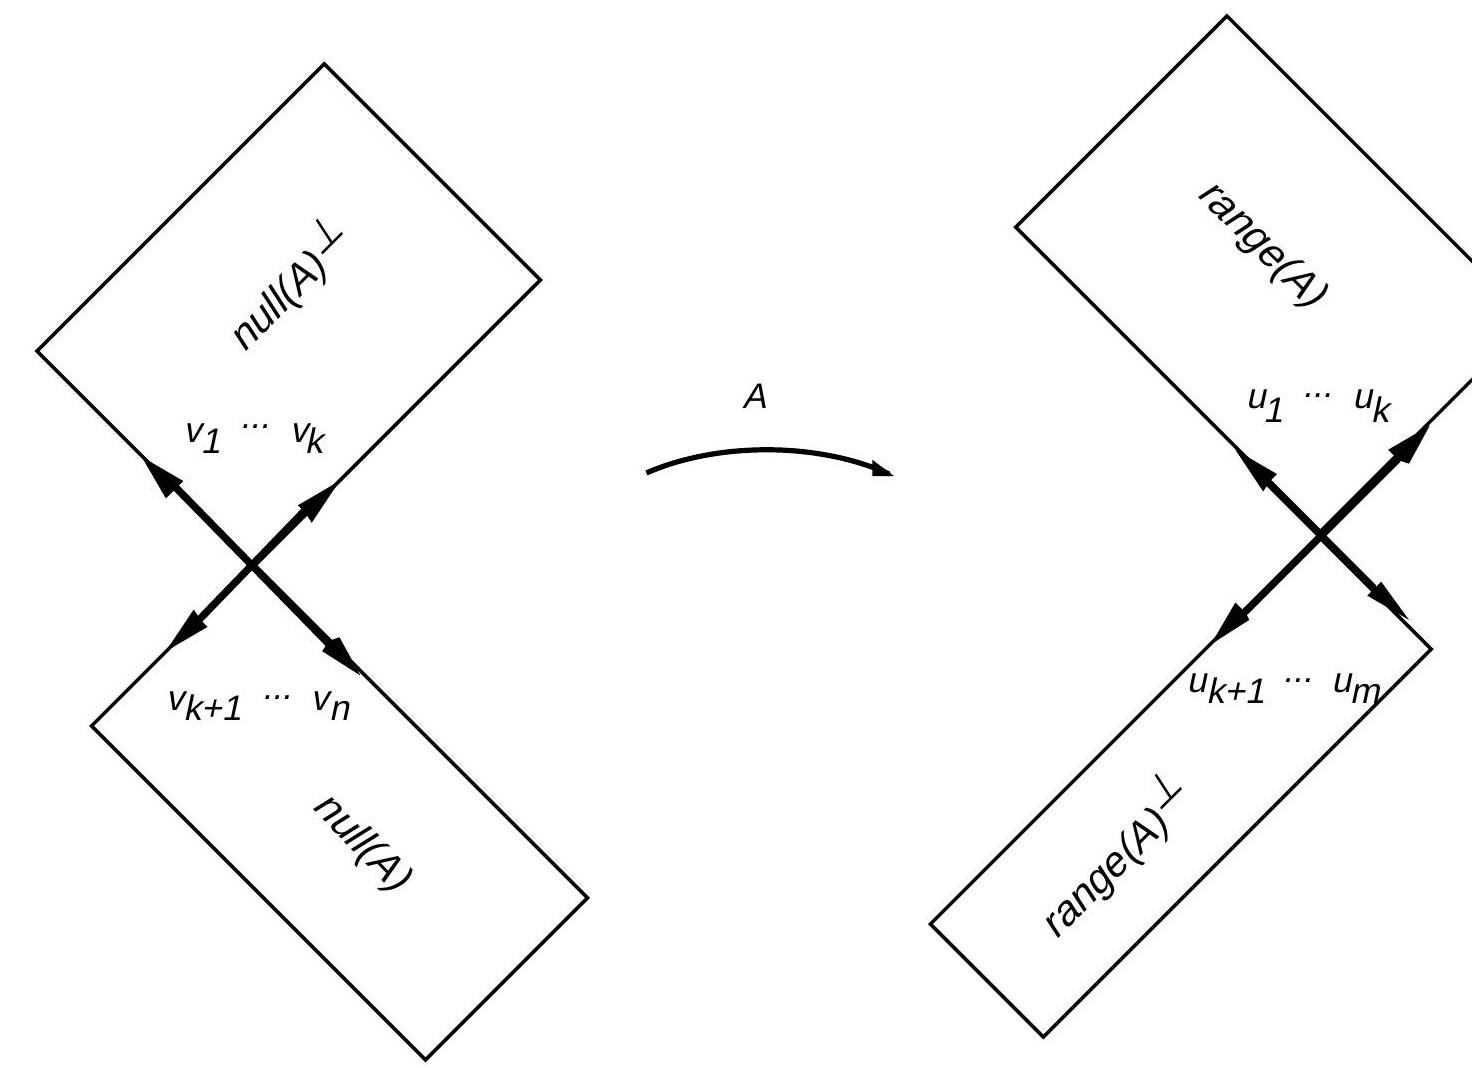
\includegraphics[totalheight=4in]{./fig/1.jpg}
  \caption{Strang's Diagram} 
  \label{fig:1}
\end{figure}

现在让我们继续讨论 SVD 的其他几个方面。

\subsection{SVD 和 EVD}
我们的构造展示了如何从对称矩阵 $A^{T} A$ 的 EVD 确定 A 的 SVD。相反,很容易从$A$的SVD中恢复$A^{T}A$的EVD。假设给定奇异值分解 $A=U \Sigma V^{T}$。显然,$A^{T} A=V \Sigma^{T} \Sigma V^{T}$ 和 $A A^{T}=U \Sigma \Sigma^{T} U^{T}$。现在在任一顺序中,$\Sigma$ 和 $\Sigma^{T}$ 的乘积是一个正方形对角矩阵,其前 k 个对角线元素是 $\sigma_{i}^{2}$,并且任何剩余的对角线元素等于 0 。因此,$A^{T} A=V \Sigma^{T} \Sigma V^{T}$ 是 $A^{T} A$的 EVD 且 $A A^{T}=U \Sigma \Sigma^{T} U^{T}$ 是 $A A^{T}$ 的 EVD。我们的论点还为奇异值分解产生了唯一性结果。在 $A$ 的任何 SVD 中,右奇异向量($V$ 的列)必须是 $A^{T} A$ 的特征向量,左奇异向量($U$ 的列)必须是 $ A A^{T}$的特征向量,并且奇异值必须是这两个对称矩阵共有的非零特征值的平方根。因此,直到$A^{T} A$ 和$A A^{T}$ 的多维特征空间中可能的正交变换,SVD 中的矩阵$V$ 和$U$ 是唯一确定的。最后,请注意,如果 $A$ 本身是正方形且对称的,则具有特征值 $\lambda$ 的 $A$ 的每个特征向量都是 $A^{2}=A^{T} A=A A^{T}$ 的特征向量具有特征值 $\lambda^{2}$。因此,$A$ 的左右奇异向量只是 $A$ 的特征向量,$A$ 的奇异值是其特征值的绝对值。也就是说,对于对称的 $A$,EVD 和 SVD 基本一致,如果 $A$ 没有负特征值,它们实际上是相同的。特别是,对于任何 $A$,$A^{T} A$ 的 SVD 和 $\mathrm{EVD}$ 是相同的。

\subsection{SVD 的几何解释}
理解 $A$ 如何使空间变形的一种方法是考虑它在 $\mathbf{R}^{\mathbf{n}}$ 中的单位球面上的作用。 该单位球面的任意元素 $x$ 可以表示为 $x=x_{1} v_{1}+x_{2} v_{2}+\cdots+x_{n} v_{n}$ 和 $\sum_{1}^{n} x_{i}^{2}=1$。 图像是 $A x=\sigma_{1} x_{1} u_{1}+\cdots+\sigma_{k} x_{k} u_{k}$。 令$y_{i}=x_{i} \sigma_{i}$,我们看到单位球体的图像由向量$y_{1} u_{1}+y_{2} u_{2}+\cdots+y_{k} u_{k}$,其中
$$
\begin{aligned}
\frac{y_{1}^{2}}{\sigma_{1}^{2}}+\frac{y_{2}^{2}}{\sigma_{2}^{2}}+\cdots+\frac{y_{k}^{2}}{\sigma_{k}^{2}} &=\sum_{1}^{k} x_{i}^{2} \\
& \leq 1
\end{aligned}
$$

如果$A$ 具有满列秩,因此$k=n$,则不等式实际上是严格等式。 否则,右边的一些 $x_{i}$ 会丢失,总和可以是 0 到 1 之间的任何值。 这表明 $A$ 将 $\mathbf{R}^{\mathbf{n}}$ 的单位球面映射到 $k$ 维椭球,半轴在 $u_{i}$ 方向上,并且 幅度 $\sigma_{i}$。 如果$k=n$,图像只是椭球的表面,否则就是实心椭球。 综上所述,我们可以将 $A$ 的效果可视化如下:它首先折叠域的 $n-k$ 个维度,然后扭曲剩余的维度,将单位 $k$-sphere 拉伸和挤压成一个椭球体,最后将椭球体嵌入到 $\mathbf{R}^{\mathbf{m}}$。 这在图 (\ref{fig:2}) 中对 $n=m=3$ 和 $k=2$ 进行了说明。

\begin{figure}[htbp]%[htbp]
  \centering
  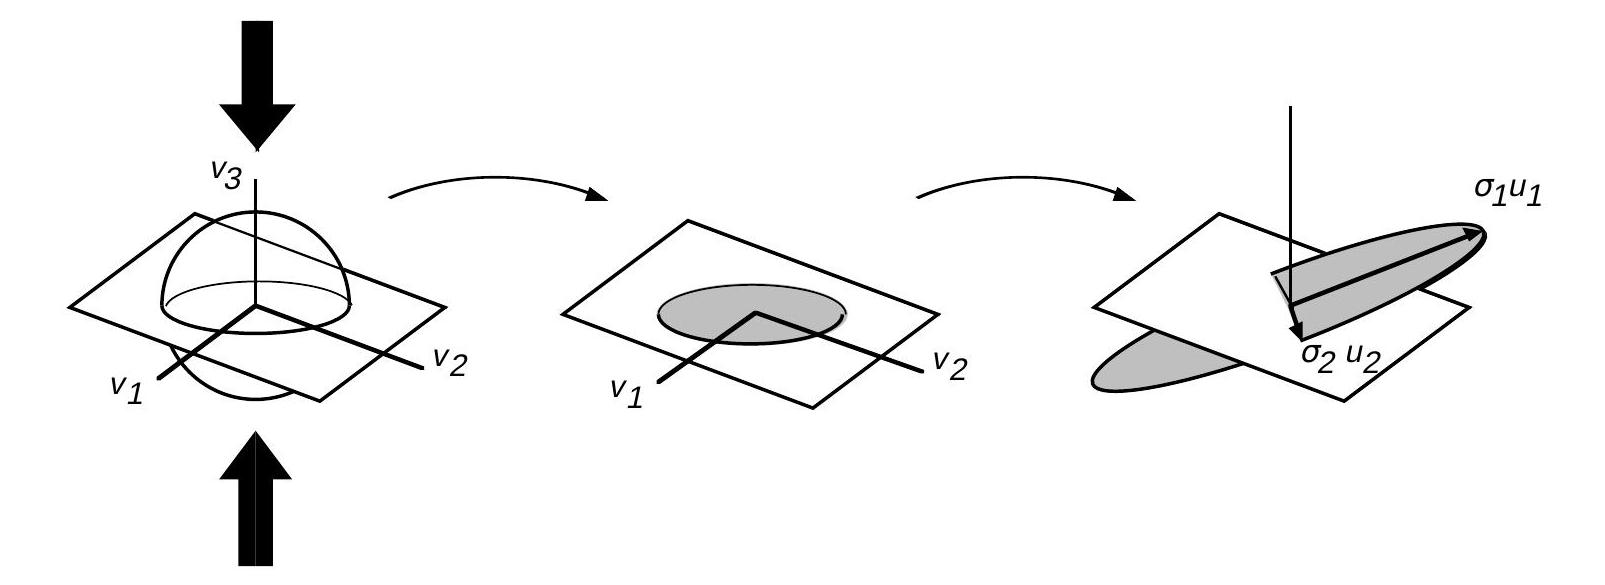
\includegraphics[totalheight=2.5in]{./fig/2.jpg}
  \caption{$A$ 如何变形到 $\mathbf{R}^{\mathbf{n}}$} 
  \label{fig:2}
\end{figure}

作为直接结果,我们看到 $\|A\|$,$A$ 的算子范数,定义为单位球面上 $v$ 的 $|A v|$ 的最大值,就是 $\sigma_ {1}$,$A$ 的最大奇异值。 换句话说,我们有不等式 $|A x| \leq \sigma_{1}|x|$ 对于所有 $x \in \mathbf{R}^{\mathbf{n}}$,只有当 $x$ 是 $v_{1}$ 的倍数时才相等。

\subsection{分区矩阵和 SVD 的外积形式}
从纯代数的角度来看,矩阵 $\Sigma$ 的任何零行和零列都是多余的。 如果矩阵乘积 $A=U \Sigma V^{T}$ 使用分区矩阵表示,则可以消除它们,如下所示
$$
A=\left[\begin{array}{lll|lll}
u_{1} & \cdots & u_{k} & u_{k+1} & \cdots & u_{m}
\end{array}\right]\left[\begin{array}{ccc|c}
\sigma_{1} & & & \\
& \ddots & & 0 \\
& & \sigma_{k} & \\
\hline & 0 & & 0 \\
& & &
\end{array}\right]\left[\begin{array}{c}
v_{1}^{T} \\
\vdots \\
v_{k}^{T} \\
\hline v_{k+1}^{T} \\
\vdots \\
v_{n}^{T}
\end{array}\right]
$$
尽管这些分区假设 $k$ 严格小于 $m$ 和 $n$,但如果 $k$ 等于 $m$ 或 $n$,应该清楚如何修改参数。 当划分的矩阵相乘时,结果是
$$
A=\left[\begin{array}{lll}
u_{1} & \cdots & u_{k}
\end{array}\right]\left[\begin{array}{ccc}
\sigma_{1} & & \\
& \ddots & \\
& & \sigma_{k}
\end{array}\right]\left[\begin{array}{c}
v_{1}^{T} \\
\vdots \\
v_{k}^{T}
\end{array}\right]+\left[\begin{array}{lll}
u_{k+1} & \cdots & u_{m}
\end{array}\right]
\begin{Huge}
\left[\begin{array}{ccc}
&
\mathbf{0} &
\\
\end{array}\right]
\end{Huge}
\left[\begin{array}{c}
v_{k+1}^{T} \\
\vdots \\
v_{n}^{T}
\end{array}\right]
$$

从最后一个等式可以清楚地看出,只有前 $k$个$u$ 和 $v$ 对 $A$ 有贡献。 事实上,我们不妨将方程缩短为
$$
A=\left[\begin{array}{lll}
u_{1} & \cdots & u_{k}
\end{array}\right]\left[\begin{array}{ccc}
\sigma_{1} & & \\
& \ddots & \\
& & \sigma_{k}
\end{array}\right]\left[\begin{array}{c}
v_{1}^{T} \\
\vdots \\
v_{k}^{T}
\end{array}\right]
$$

请注意,在这种形式中,$u$ 和 $v$ 的矩阵现在是矩形的(分别为 $m \times k$ 和 $k \times n$),并且对角矩阵是正方形。 这是 SVD 的另一种版本,在某些说明中被用作定义:任何秩为 $k$ 的 $m \times n$ 矩阵 $A$ 都可以表示为 $A=U \Sigma V^{T }$ 其中 $U$ 是一个 $m \times k$ 矩阵,使得 $U^{T} U=I, \Sigma$ 是一个 $k \times k$ 对角矩阵,其正项在对角线上按降序排列, $V$ 是一个 $n\times k$ 矩阵,使得 $V^{T} V=I$。

SVD 的分区矩阵公式在某一方面有点不寻常。 通常在矩阵乘积 $X Y$ 中,我们关注 $X$ 中的行和 $Y$ 中的列。 在这里,因子以相反的方式表达。 这是对两个矩阵的乘积应用所谓的外积展开的理想情况。 一般来说,如果 $X$ 是一个 $m \times k$ 矩阵,列 $x_{i}$ 和 $Y$ 是 $k \times n$ 矩阵,行 $y_{i}^{T}$, 矩阵积 $X Y$ 可以表示为
$$
X Y=\sum_{i=1}^{k} x_{i} y_{i}^{T}
$$
每个项 $x_{i} y_{i}^{T}$ 是向量 $x_{i}$ 和 $y_{j}$ 的外积。 它只是列矩阵和行矩阵的标准矩阵乘积。 结果可以用乘法表来可视化,$x_{i}$ 的条目列在左边距,$y_{j}$ 的条目列在顶部。 表的主体是 $x_{i}$ 和 $y_{j}$ 的外积。 这个想法如图(\ref{fig:3})所示,显示了$(a,b,c)$和$(p,q,r)$的外积。 观察图中,每一列都是$\left[\begin{array}{l}a \\ b \\ c\end{array}\right]$的倍数,每一行都是 $\left[\begin{array}{ccc}p & q & r\end{array}\right]$ 的倍数,因此外积显然是秩1。以同样的方式, 外积 $x_{i} y_{i}^{T}$ 是一个秩为 1 的矩阵,其列是 $x_{i}$ 的倍数,行是 $y_{i}$ 的倍数。
\begin{figure}[htbp]
\centering
\begin{tabular}{c|ccc}
 & $p$ & $q$ & $r$ \\
\hline
$a$ & $a p$ & $a q$ & $a r$ \\
$b$ & $b p$ & $b q$ & $b r$ \\
$c$ & $c p$ & $a q$ & $c r$ \\
\end{tabular}
\caption{外积为乘法表}
\label{fig:3}
\end{figure}

我们将在 SVD 的一种应用中返回到外积扩展。 在这里,我们简单地应用这个概念来以不同的形式表达 A 的 SVD。

令
$$
X=\left[\begin{array}{lll}
u_{1} & \cdots & u_{k}
\end{array}\right]\left[\begin{array}{ccc}
\sigma_{1} & & \\
& \ddots & \\
& & \sigma_{k}
\end{array}\right]=\left[\begin{array}{ccc}
\sigma_{1} u_{1} & \cdots & \sigma_{k} u_{k}
\end{array}\right]
$$
且
$$
Y=\left[\begin{array}{c}
v_{1}^{T} \\
\vdots \\
v_{k}^{T}
\end{array}\right]
$$
那么$A=X Y$可以表示为外积展开
$$
A=\sum_{i=1}^{k} \sigma_{i} u_{i} v_{i}^{T}
$$
这是 SVD 的另一种形式,它提供了另一种表达 $A$ 如何转换任意向量 $x$ 的方式。 清楚地,
$$
A x=\sum_{i=1}^{k} \sigma_{i} u_{i} v_{i}^{T} x
$$
由于 $v_{i}^{T} x$ 是一个标量,我们可以将因子的顺序重新排列为
$$
A x=\sum_{i=1}^{k} v_{i}^{T} x \sigma_{i} u_{i}
$$

在这个和中,$A x$表示为向量$u_{i}$的线性组合。每个系数是两个因子$v_{i}^{T} x$和$\sigma_{i}$的乘积。当然,$v_{i}^{T} x=v_{i} \cdot x$只是$x$相对于正交基$\left\{v_{1}, \cdots, v_{n}\right\}$的$i^{\text {th}}$分量。从这个角度来看,外积扩展再次确认了我们已经知道的:在$A$的作用下,$x$的每个$v$分量在按适当的$\sigma$缩放后变成$u$分量。

\section{应用}
通常,SVD 可应用于涉及大型矩阵的问题,其维度可以达到数千。正是存在用于计算的高效和准确的计算机算法,才使得 SVD 在这些应用中如此有用。算法的推导涉及美丽的数学,这个主题值得研究。然而,对于目前的应用讨论,我们将 SVD 的计算视为由黑盒执行。通过类比,考虑三角学的任何应用。当我们需要正弦或余弦的值时,我们只需按下计算器上的按钮,而无需考虑内部工作原理。我们相信计算器会返回一个足够接近的近似值来满足我们的目的,并且不再考虑它。因此,在目前的讨论中,让读者相信计算机可以快速准确地逼近任意矩阵的 SVD。为了扩展类比,我们将集中讨论何时以及为什么按下 SVD 按钮,以及如何使用结果。

SVD 是多种不同应用中的重要工具。 在这里,我们将详细讨论两个显然完全不相关的样本:线性最小二乘优化和降低秩近似的数据压缩。 在继续讨论这些主题之前,将简要介绍一些其他应用程序。

\subsection{应用简介}
SVD 最直接的应用之一是计算矩阵积 $A^{T} A$ 的 EVD。 这类问题经常以主成分分析\footnote{[15,第 8 章]的介绍部分描述了数字图像处理的应用。 随后的部分讨论了 SVD 及其其他应用。 关于图像处理的更详细的介绍出现在 [21,第 6 章]。} 的名义出现,并且在与协方差矩阵分析 \footnote{例如,参见 [9]。} 相关的统计中经常遇到。 正如对最小二乘优化的讨论将表明的那样,$A^{T}A$ 的计算会导致结果准确性的显着下降。 相反,可以通过直接对原始矩阵 $A$ 进行运算来计算 SVD。 这给出了 $A^{T} A$ 的所需特征向量($A$ 的右奇异向量)和 $A^{T} A$ 的特征值($A$ 的奇异值的平方),而无需明确 计算 $A^{T} A$。

作为第二个应用,SVD 可以用作矩阵有效秩的数值可靠估计。 通常,数据中的线性相关性被测量误差所掩盖。 因此,尽管从计算上讲,数据矩阵的列似乎是线性独立的,但通过完美的测量,可以检测到相关性。 或者,换一种说法,可以通过少量扰动条目来使数据矩阵的列依赖,其顺序与数据中已经存在的测量误差相同。 找到这些依赖关系的方法是关注比测量误差更大的奇异值。 如果存在$r$这样的奇异值,则发现矩阵的有效秩为$r$。 这个主题与选择最接近矩阵的秩近似的想法密切相关,在数据压缩的讨论中进一步考虑了这一点。

SVD 的第三个应用是计算所谓的矩阵的广义逆。 这与线性最小二乘问题密切相关,将在该主题的讨论中再次提及。 然而,由于广义逆的主题本身就很有趣,因此在 SVD 的应用中值得在这里简要提及。

简要提到的应用程序列表到此结束。 接下来我们继续详细研究至少二乘问题。

\subsection{线性最小二乘}
线性最小二乘问题的一般背景是这样的:我们有一组向量,我们希望将它们线性组合以提供给定向量的最佳可能近似值。 如果向量集是 $\left\{a_{1}, a_{2}, \cdots, a_{n}\right\}$ 并且给定向量是 $b$,我们寻求系数 $x_{1} , x_{2}, \cdots, x_{n}$ 产生最小误差
$$
\left|b-\sum_{i=1}^{n} x_{i} a_{i}\right|
$$
这个问题可以在任何向量空间中自然出现,其中的元素是序列、函数、微分方程的解等。 只要我们只对有限集 $\left\{a_{1}, a_{2}, \cdots, a_{n}\right\}$ 的线性组合感兴趣,就可以将问题转化为 一种涉及有限列的数字。 在这种情况下,定义一个矩阵 $A$,其列由 $a_{i}$ 给出,以及一个向量 $x$,其条目是未知系数 $x_{i}$。 然后我们的问题是选择 $x$ 最小化 $|b-A x|$。 和前面的讨论一样,我们将用 $m$ 和 $n$ 来表示 $A$ 的维度,这意味着在这种情况下 $a_{i}$ 是长度为 $m$ 的向量。

一般最小二乘问题有一个几何解释。 我们正在寻找由 $a_{i}$ 跨越的子空间 $S$ 中最接近 $b$ 的元素。 解是$b$在$S$上的投影,其特征是误差向量(即$b$与其投影之间的向量差)应该与$S$正交。 与 $S$ 的正交性等同于与每个 $a_{i}$ 的正交性。 因此,对于所有 $i$,最优解向量 $x$ 必须满足 $a_{i} \cdot(A x-b)=0$。 等效地,在矩阵形式中,$A^{T}(A x-b)=0$。

将方程改写为$A^{T} A x=A^{T} b$,$x_{i}$ 的一组方程通常称为线性最小二乘问题的正规方程。 观察 $A$ 列的独立性意味着 $A^{T} A$ 的可逆性。 因此,我们有 $x=\left(A^{T} A\right)^{-1} A^{T} b$。

这是一个美丽的分析。 它整洁,优雅,清晰。 不幸的是,当它以近似计算机算术实现时,它的表现也很差。 事实上,这是前面提到的理论与实践之间差距的典型例子。 在数值上,$A^{T} A$ 的形成会极大地降低计算的准确性; 这是一个需要避免的步骤。 [8] 中详细讨论了这种性能不佳的原因。 在这里,我们将满足于使用启发式分析和数值示例来深入了解问题。 不过,首先让我们看看 SVD 如何解决最小二乘问题。

我们要选择向量$x$ 以最小化$|A x-b|$。 令 $A$ 的 $\mathrm{SVD}$ 为 $U \Sigma V^{T}$(其中 $U$ 和 $V$ 是正交正交矩阵,$\Sigma$ 是与 $A)$。 然后我们有
$$
\begin{aligned}
A x-b &=U \Sigma V^{T} x-b \\
&=U\left(\Sigma V^{T} x\right)-U\left(U^{T} b\right) \\
&=U(\Sigma y-c)
\end{aligned}
$$
其中 $y=V^{T} x$ 和 $c=U^{T} b$。 现在 $U$ 是一个正交矩阵,因此保留了长度。 也就是说,$|U(\Sigma y-c)|=|\Sigma y-c|$,因此 $|A x-b|=|\Sigma y-c|$。 这提出了一种解决最小二乘问题的方法。 首先,确定$A$ 的SVD 并计算$c$ 作为$U^{T}$ 和$b$ 的乘积。 接下来,求解 $\Sigma$ 和 $c$ 的最小二乘问题。 也就是说,找到一个向量 $y$ 使得 $|\Sigma y-c|$ 是最小的。 (稍后我们将看到$\Sigma$ 的对角线性质使这一步变得微不足道。)现在$y=V^{T} x$ 所以我们可以确定$x$ 为$V y$。 这给出了解向量 $x$ 以及误差的大小 $|\Sigma y-c|$。

实际上,SVD 允许我们改变变量,从而将最小二乘问题简化为对角线形式。 在这种特殊形式下,很容易得到解决方案。 我们寻求 $y$ 以最小化向量 $\Sigma y-c$ 的范数。 令$\Sigma$ 的非零对角项为$\sigma_{i}$,对于$1 \leq i \leq k$,令$y$(即未知数)的分量为$y_{i}$,对于 $1 \leq i \leq n$。 然后
$$
\Sigma y=\left[\begin{array}{c}
\sigma_{1} y_{1} \\
\vdots \\
\sigma_{k} y_{k} \\
0 \\
0 \\
\vdots \\
0
\end{array}\right] \text { so } \quad \Sigma y-c=\left[\begin{array}{c}
\sigma_{1} y_{1}-c_{1} \\
\vdots \\
\sigma_{k} y_{k}-c_{k} \\
-c_{k+1} \\
-c_{k+2} \\
\vdots \\
-c_{m}
\end{array}\right]
$$
通过检查,当 $y_{i}=c_{i} / \sigma_{i}$ for $1 \leq i \leq k$ 时,$\Sigma y-c$ 假定其最小长度,由下式给出
\begin{align}
\left[\sum_{i=k+1}^{m} c_{i}^{2}\right]^{1 / 2}
\end{align}
请注意,当 $k=m$ 时,总和是空的。 在这种情况下,$A$ 的列跨越 $\mathbf{R}^{\mathbf{m}}$,因此可以以零误差解决最小二乘问题。 还观察到当$k$ 小于$n$ 时,$y_{k+1}$ 到$y_{n}$ 的值没有约束。 可以为这些组件分配任意值,而不影响 $\Sigma y-c$ 的长度。

正如前面的分析所示,SVD 允许我们将一般最小二乘问题转换为可以通过检查解决的问题,而对数据矩阵 $A$ 的秩没有限制。 实际上,我们可以将转换步骤和简化问题的解决方案组合如下。 首先,我们知道$c=U^{T} b$。 从 $c$ 计算 $y$ 等于乘以矩阵 $\Sigma^{+}$,通过转置 $\Sigma$ 和反转非零对角项来定义。 然后 $y=\Sigma^{+} c$ 将根据需要将其前 $k$ 个条目等于 $c_{i} / \sigma_{i}$。 任何剩余的元素(以前不受约束)都消失了。 最后,我们计算 $x=V y$。 这给出了紧凑的解决方案
\begin{align}
x=V \Sigma^{+} U^{T} b
\end{align}

至此,广义逆曲面的主题。 给定 $b \in \mathbf{R}^{\mathbf{m}}$,有一个唯一元素 $x \in \mathbf{R}^{\mathbf{n}}$ 满足 $A x$ 最接近 $b$。 从 $b$ 到 $x$ 的映射定义了 $A$ 的所谓 Moore-Penrose 广义逆 $A^{+}$。 很明显,$\Sigma^{+}$,如 $\Sigma$ 和 $c$ 的租约平方问题的解中所定义,是 $\Sigma$ 的 Moore-Penrose 逆。 此外,方程式(2) 表明当$A=U \Sigma V^{T}$ 是$A$ 的SVD 时,广义逆由$A^{+}=V \Sigma^{+} U^{T }$。 在 [5] 中给出了对紧凑和自包含的广义逆的很好处理,尽管在该工作中没有提到 SVD。 $[8,14,22,23]$ 中还讨论了广义逆及其与 SVD 的联系。

现在我们可以比较使用 SVD 和正规方程获得的解。 这些解在理论上是等价的,所以如果它们以精确的算术进行,它们必须产生相同的结果。 但是当在计算机上以有限的精度执行时,它们可能会有很大的不同。 这种差异的核心在于舍入误差的影响。 因此,在继续之前,我们暂停考虑舍入误差的一个重要方面。

一个例子将使这方面变得清晰。 设 $x=1.23456789012345 \cdot 10^{8}$ 和 $y=1.23456789012345$。 $10^{-1}$。 用 15 个正确数字计算,$x$ 和 $y$ 的总和由下式给出
$$
\begin{array}{rll}
12345678 & 9012345 \\
+\quad . & 123456789012345 \\
\hline 12345679 . & 0246912
\end{array}
$$
这对应于在 $y$ 的小数点 $8^{\text {th }}$ 处引入错误。 请注意,虽然每个数字在计算机中以 15 位小数的精度表示,但一个术语的最低有效数字基本上没有意义。 如果这两项在幅度上相差足够大(在示例中为 16 个数量级),则较小项的贡献将被完全消除。

当系统矩阵的奇异值在幅度上变化很大时,这个问题就会出现在线性系统的反演中。 例如,考虑作为正规方程的一部分出现的 $A^{T} A$ 的反演。 正规方程公式要求 $A^{T} A$ 是非奇异的。 如果接近奇异,$A^{T} A$ 将具有非常接近 0 的奇异值,这就是正规方程变得不可靠的时候。 让我们将 $A^{T} A$ 的奇异值按降序写为 $\lambda_{1}, \lambda_{2}, \cdots, \lambda_{n}$。 这些实际上是 $A^{T} A$ 的特征值(如前所述),它们是 $A$ 奇异值的平方。 $A^{T} A$ 的特征向量是 $v_{1}, v_{2}, \cdots, v_{n}$,$A$ 的右奇异向量。 当 $\lambda_{n}$ 非常接近 0 时,$\lambda_{i}$ 很可能会覆盖很宽的量级。

为了戏剧化这种情况,我们假设 $\lambda_{n}$ 比 $\lambda_{1}$ 小几个数量级,而另一个 $\lambda_{i}$ 大致与 $\lambda_{ 1}$ 的数量级。在几何上,$A^{T} A$ 将 $\mathbf{R}^{\mathbf{n}}$ 的单位球面映射到一个椭球体上,其轴在 $v_{i}$ 的方向上。 $v_{n}$ 方向上的轴长度比所有其他轴小得多,以至于椭圆体看起来完全变平并位于 $n-1$ 维超平面中(见图(\ref{fig:4}) )。因此,在单位长度随机向量$A^{T}A$下的图像中,$v_{n}$分量的预期贡献基本上可以忽略不计。在这种情况下,有限精度的影响是在$v_{n}$ 的贡献中引入了显着的误差。然而,在求解正规方程时,我们对逆映射感兴趣,$\left(A^{T} A\right)^{-1}$,它具有与 $A^{T} A$ 相同的特征向量,但其特征值是倒数 $1 / \lambda_{i}$。现在只有$\lambda_{n}$ 是重要的,并且椭圆体本质上是一维的(见图(\ref{fig:5}))。在除$v_{n}$ 之外的每个方向上,随机单位向量的图像都没有显着的贡献。如前所述,除$v_{n}$ 之外的所有$v_{i}$ 的贡献都引入了重大误差。

\begin{figure}[htbp]%[htbp]
  \centering
  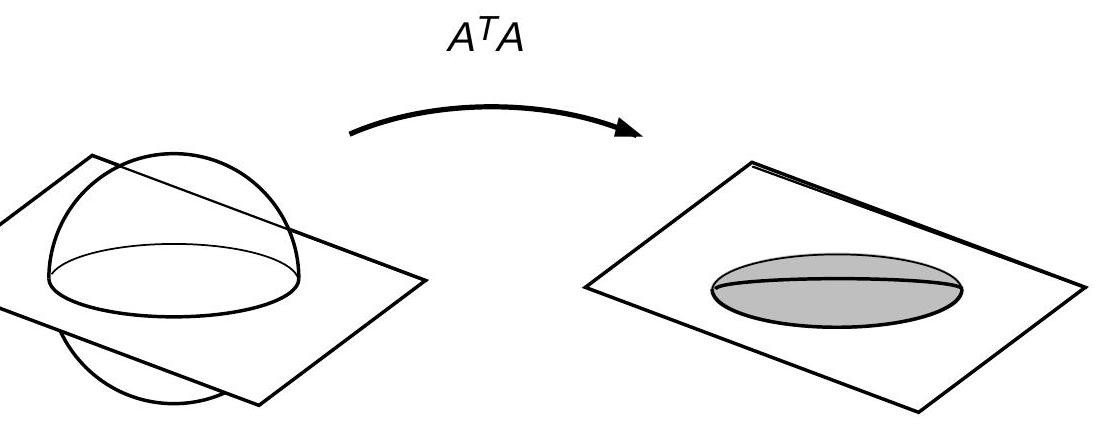
\includegraphics[totalheight=2in]{./fig/4.jpg}
  \caption{由 $A^{T} A$ 变形的单位球体} 
  \label{fig:4}
\end{figure}

\begin{figure}[htbp]%[htbp]
  \centering
  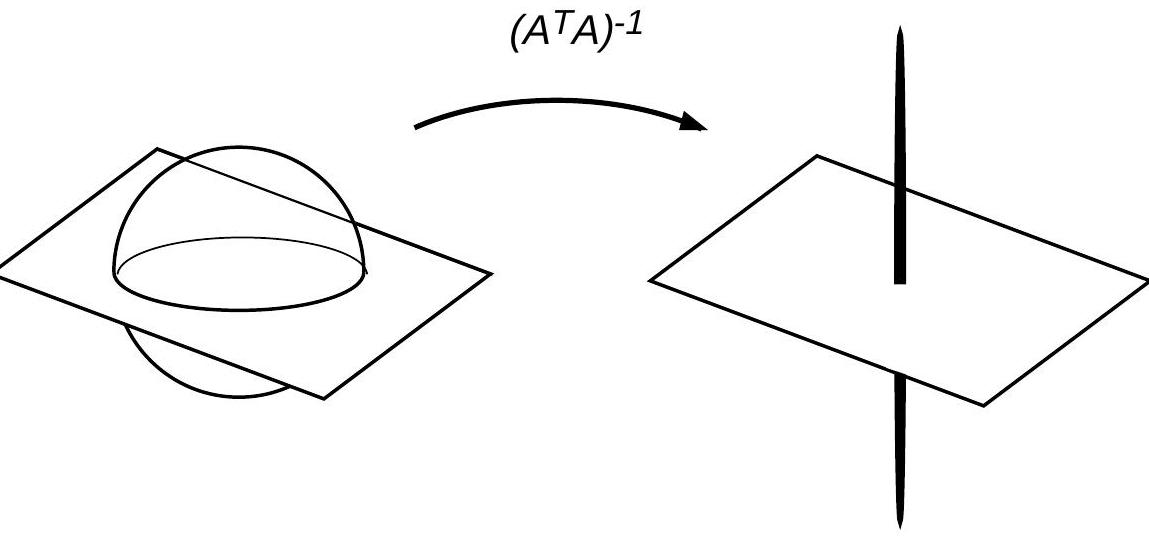
\includegraphics[totalheight=2in]{./fig/5.jpg}
  \caption{由 $\left(A^{T} A\right)^{-1}$ 变形的单位球体} 
  \label{fig:5}
\end{figure}

让我们更具体地分析一下。让一个特定的向量 $x$ 被选中,其中 $x=x_{1} v_{1}+$ $x_{2} v_{2}+\cdots+x_{n} v_{n}$。将 $x$ 视为列向量,考虑单个条目 $c$,并为 $x_{i} v_{i}$ 的相应条目写入 $c_{i}$。那么$c=c_{1}+c_{2}+\cdots+c_{n}$。在图像 $\left(A^{T} A\right)^{-1} x$ 中,对应的条目将是 $c_{1} / \lambda_{1}+c_{2} / \lambda_{2} +\cdots+c_{n} / \lambda_{n}$。现在,如果 $c_{i}$ 的大小都大致相当,那么最后一项将使其余项相形见绌。会出现上述情况。 $c_{n} / \lambda_{n}$ 项将扮演 $12345678.9012345$ 的角色;每隔一个术语将在 123456789012345 的位置。实际上,每个术语的几个十进制数字,除了最后一个,都被忽略了。当然,忽略的位数取决于 $\lambda_{1}$ 和 $\lambda_{n}$ 之间的大小差异。如果 $\lambda_{1} / \lambda_{n}$ 在 $10^{\tau}$ 的数量级上,则 $\lambda_{1}$ 和 $\lambda_{n}$ 相差 $\tau$ 个数量级量级,并且总和的次等项损失了 $\tau$ 位的准确性。如果$\tau$足够大,除了最后一项外,每一项的贡献都可能完全丢失。

这种准确性的损失真的很重要吗? $y=\left(A^{T} A\right)^{-1} x$ 的值对计算的准确性是否仍然正确? 如果 $y$ 真的是我们所关心的,是的。 但是$y$应该是$A^{T} A y=x$的近似解,我们应该通过观察$A^{T} A y$和$之间的差异来判断这个近似的充分性 x$。 在精确的算术中,在计算 $y$ 时几乎可以忽略的第一个 $n-1 c_{i} / \lambda_{i}$ 重新获得了它们的意义,并对 $x$ 的恢复做出了重要贡献。 但是在有限精度算法中丢失的数字无法恢复,因此除了最后一个之外,每个元素要么被破坏,要么完全丢失。 因此,虽然 $y=\left(A^{T} A\right)^{-1} x$ 可能对计算精度的限制是正确的,但 $A^{T} A y$ 的计算值可以是每个小数位都不正确。

在正规方程的上下文中,$x=\left(A^{T} A\right)^{-1} A^{T} b$ 的计算应该导致乘积 $A x$ 接近到$b$。 此计算会出现与上述相同的错误。 $\left(A^{T} A\right)^{-1}$ 计算中的小错误可能会因最终乘以 $A$ 而膨胀,从而严重降低最终结果的准确性。

综上所述,$A^{T} A$的特征值的大小决定了在计算最小二乘向量$x$时有限精度的影响,当$\lambda_{1} / \lambda_{n}$较大时,这些影响最为严重。 正如许多读者会认识到的,这个比率是矩阵 $A^{T} A$ 的条件数。 更一般地,对于任何矩阵,条件数是最大奇异值与最小奇异值之比。 对于方阵 $A$,条件数可以解释为到最近奇异矩阵的距离的倒数 ([8, p. 26])。 矩阵的大条件数表明数值不稳定性可能会困扰许多类型的计算,尤其是线性系统的解。

现在所有这些讨论同样适用于最小二乘问题的 SVD 解决方案。我们也必须反转一个矩阵,将 $U^{T} b$ 乘以 $\Sigma^{+}$。实际上,奇异值是显式反转的,我们可以看到最小正奇异值方向上的分量被膨胀,在非奇异情况下,因子 $1 / \sigma_{n}$。如前所述,当条件数 $\sigma_{1} / \sigma_{n}$ 很大时,会感受到截断的影响。因此,SVD 解决方案的好处不是避免了 $A$ 列的近依赖效应。但是让我们比较两个条件数。我们知道$A^{T} A$ 的特征值是$A$ 的奇异值的平方。因此$\lambda_{1} / \lambda_{n}=\left(\sigma_{1} / \sigma_{n}\right)^{2}$,$A^{T} A$ 的条件数为$A$ 的条件数的平方。鉴于我们的启发式错误分析,条件数之间的这种关系解释了数值计算的经验法则:使用 $A^{T} A$ 的计算需要使用大约两倍的数字来执行,以确保最终结果其准确性与 $A$ 的 SVD 提供的准确性相当。

启发式分析是合理的,但其本身并不能完全令人信服。 以下数值示例提供了一些支持启发式论证的证据。 当然,仔细的数学分析是不可替代的,有兴趣的读者可以参考 $[8]$ 来讨论条件数。

\subsection{数值示例}
我们将模拟最小二乘分析,其中已经收集了四个变量的实验数据,并且我们试图通过其他三个自变量的线性组合来估计一个,即因变量。为简单起见,我们假设每个变量仅由四个数据值指定,因此 $A$ 的列 $a_{1},a_{2},a_{3}$ 以及依赖列 $b$ 位于$\mathbf{R}^{4}$.我们希望 $A$ 的列几乎是相关的,以便我们可以观察启发式分析中描述的情况。这将通过使一列(例如 $a_{3}$)与其他两列的线性组合相差一个非常小的随机向量来实现。同样,我们希望从属向量 $b$ 接近但不在 $A$ 的范围内,因此我们也将其定义为 $a_{1}$ 和 $a_{2} $ 的线性组合加上一个小的随机向量。然后我们用$x=V \Sigma^{+} U^{T} b$和$x=\left(A^{T} A\right)^{-1} A^{T} b$两个公式计算最小二乘系数$x=\left(x_{1}, x_{2}, x_{3}\right)$,并通过计算每种情况下残差$| -A x|$的大小来比较误差。

在 $a_{3}$ 和 $b$ 的定义中选择随机向量时,我们有不同的目标。 $b$ 的随机分量将决定 $b$ 与 $A$ 的范围相距多远,因此我们应该从最小二乘解中观察到多大的残差。我们所有的计算都将精确到小数点后 16 位。考虑到这一点,我们将 $b$ 的随机分量相当小,大约为 $10^{-4}$。相反,选择$a_{3}$ 的随机分量的目标是使$A$ 的条件数在$10^{8}$ 的量级上。那么 $A^{T} A$ 的条件数将在 $10^{16}$ 的数量级上,大到足以破坏由正规方程产生的解的所有 16 位十进制数字。正如我们稍后关于降秩近似的讨论中所展示的,$A$ 的最小奇异值将与用于定义 $a_{3}$ 的随机向量的范数大致相同。如果 $a_{1}$ 和 $a_{2}$ 的范数在 10 的数量级上,那么最大的奇异值也将是。因此,选择 $b$ 的随机分量,范数约为 $10^{-7}$ 应该会产生所需范围内的条件数。

在这一点上值得注意的是,$A$ 列之间的近似相关性不应降低最小二乘解的质量。 仅使用 $A$ 的前两列,就可以将 $b$ 近似为大约 $10^{-4}$ 的误差。 $A$ 的第三列只能提高近似值。 因此,应该期望真正的最小二乘解产生不大于 $10^{-4}$ 的残差。 因此,使用正规方程获得的大误差完全归因于算法的数值不稳定性,而不是最小二乘问题的任何内在限制。

本例中的所有计算均使用计算机软件包 MATLAB [18] 进行。 它用于定义和操作矩阵的简单程序使得这种探索几乎毫不费力。 鼓励读者进一步探索该主题,使用 MATLAB 重新创建和修改此处提供的示例。 为了使该过程更简单,示例的演示将包括在每个步骤中使用的确切 MATLAB 命令。 实际使用程序时,每次计算的结果都会显示在电脑屏幕上,但这里为了节省篇幅,只显示最终结果。

首先,定义两个数据向量:
\begin{lstlisting}
    c1 = [1 2 4 8]'
    c2 = [3 6 9 12]'
\end{lstlisting}
(素数表示转置运算符,因此 $\mathrm{c} 1$ 和 $\mathrm{c} 2$ 被定义为列向量。)第三个数据向量是这些的组合,加上一个非常小的随机向量 :
\begin{lstlisting}
    c3 = c1 - 4*c2 + .0000001*(rand(4,1) - .5*[1 1 1 1]')
\end{lstlisting}
并且矩阵 $A$ 被定义为将这三个向量作为其列:
\begin{lstlisting}
    A=[c1 c2 c3]
\end{lstlisting}

在 $c 3$ 的定义中,命令 rand $(4,1)$ 返回一个 4元素列向量,其中元素在 0 和 1 之间随机选择。 从每个元素中减去 $0.5$ 会使元素在 $-1 / 2$ 和 $1 / 2$ 之间移动。 因此,$c 3$ 的随机分量的长度最多为$10^{-7}$,与上面的讨论一致。

接下来,我们以类似的方式定义 $b$ 向量,将一个小的随机向量添加到 $A$ 列的指定线性组合。
\begin{lstlisting}
    b = 2*c1 - 7*c2 + .0001*(rand(4,1) - .5*[1 1 1 1]')
\end{lstlisting}

这次随机向量的长度将不大于 $10^{-4}$,再次反映了之前的讨论。

$A$ 的 SVD 由 MATLAB 快速确定:
\begin{lstlisting}
	[U,S,V] = svd(A)
\end{lstlisting}

三个矩阵 $\mathrm{U},\mathrm{S}$(代表 $\Sigma$)和 $\mathrm{V}$ 显示在屏幕上并保存在计算机内存中。 当我们运行程序时,奇异值变成了 $59.810,2.5976$ 和 $1.0578 \times 10^{-8}$。 因此 $A$ 的条件数约为 $6 \cdot 10^{9}$,并具有所需的量级。

为了计算矩阵 $\mathrm{S}^{+}$,我们需要转置对角矩阵 $\mathrm{S}$ 并反转非零对角项。 该矩阵将用 G 表示。它由以下 MATLAB 命令定义:
\begin{lstlisting}
	G = S'
	G(1,1) = 1/S(1,1)
	G(2,2) = 1/S(2,2)
	G(3,3) = 1/S(3,3)
\end{lstlisting}
现在让我们看看 SVD 解决最小二乘问题的效果如何。 我们将 $x=V \Sigma^{+} U^{T} b$ 乘以矩阵 $A$,看看结果与 $b$ 相差多远。 接到命令后
\begin{lstlisting}
	r1 = b - A*V*G*U'*b
	e1 = sqrt(r1'*r1)
\end{lstlisting}
MATLAB 返回
\begin{lstlisting}
	e1 = 4.2681e-05
\end{lstlisting}

根据需要,残差 $|b-A x|$ 的计算量值略小于 $10^{-4}$。 因此,SVD 为我们的最小二乘问题提供了令人满意的解决方案。

正规方程提供的解是$x=\left(A^{T} A\right)^{-1} A^{T} b$。 我们进入
\begin{lstlisting}
	r2 = b - A*inv(A'*A)*A'*b
	e2 = sqrt(r2'*r2)
\end{lstlisting}
且MATLAB 返回
\begin{lstlisting}
	e2 = 51.9255
\end{lstlisting}
它与$|b|$ 的数量级相同,即$b$ 到原点的距离! 正如我们从启发式分析中所预期的那样,使用正规方程计算的最小二乘问题的解决方案在将 $b$ 近似为 $A$ 列的线性组合方面做得很差。 更重要的是,这种方法计算的残差对于 $b$ 与 $A$ 范围的距离的估计没有任何价值。

这完成了我们深入研究的最小二乘问题。 下一节将详细介绍另一个应用领域:降秩近似。

\subsection{使用降秩近似的数据压缩}
前面已经介绍了用外积展开表示SVD的方法。这种表示在SVD的另一个应用——数据压缩中以一种自然的方式出现。在这个应用程序中,我们从一个$m \ n$矩阵$A$的数值数据开始,我们的目标是使用比$m n$原始条目少得多的数字来描述$A$的一个接近近似值。矩阵不被认为是一个线性变换,或者实际上根本就不是一个代数对象。它只是一个由百万美元和百万美元数字组成的表格,我们希望找到一个能捕捉到数据最重要特征的近似。

因为矩阵的秩指定线性无关的列(或行)的数量,它是冗余的度量。低秩矩阵有大量的冗余,因此可以比简单地列出所有项更有效地表达。作为一个图形的例子,假设使用扫描仪对一张照片进行数字化,用一个$m \times n$的像素矩阵替换图像,每个像素在0到1的范围内分配一个灰度级。图像中的任何大规模特征都将通过像素列或行中的冗余来反映,因此我们可能希望通过一个低于$\min (m, n)$秩的矩阵来近似地重新捕获这些特征。

极端情况是秩为 1 的矩阵。 如果 $B$ 是这样一个矩阵,那么列都是彼此的倍数 - 列空间是一维的。 如果 $u$ 是基的单个元素,则每一列都是 $u$ 的倍数。 我们将系数表示为 $v_{i}$,这意味着 $B$ 的 $i^{\text {th }}$ 列由 $v_{i} u$ 给出,因此 $B=\left[ \begin{array}{llll}v_{1} u & v_{2} u & \cdots & v_{n} u\end{array}\right]=u v^{T}$。 因此,任何一级矩阵都可以表示为外积,即列和行的乘积。 矩阵的 $m n$ 个条目由列的 $m$ 个条目和行的 $n$ 个条目决定。 出于这个原因,如果数据矩阵$A$可以近似为一个秩矩阵,我们可以实现对它的大压缩。 代替 $A$ 的 $m n$ 个条目,我们只需要 $m+n$ 个数字来表示对 $A$ 的一级近似。 寻找最佳的一级近似值是很自然的。

如果误差矩阵 $B-A$ 具有最小范数,我们将 $B$ 称为 $A$ 的最佳一级近似,现在我们将矩阵 $X$ 的 (Frobenius) 范数 $|X|$ 定义为 其元素的平方和的平方根。 这个范数只是矩阵的欧几里得范数,被视为 $\mathbf{R}^{\mathbf{m n}}$ 中的一个向量。 以这种方式考虑矩阵,两个矩阵的内积由 $X \cdot Y=\sum_{i j} x_{i j} y_{i j}$ 定义,并且像往常一样,$|X|^{2}=X \cdot X$。 显然,矩阵的这种内积可以用三种方式来理解:对应行的内积之和,对应列的内积之和,或者对应条目的 $m n$ 乘积之和。

矩阵乘积 $X Y$ 的范数有一个简单的表达式,可以使用外积展开式轻松推导出。 首先,请注意,对于第一级矩阵 $x y^{T}$ 和 $u v^{T}$,
\begin{align}
x y^{T} \cdot u v^{T}=\left[\begin{array}{lll}
x y_{1} & \cdots & x y_{n}
\end{array}\right] \cdot\left[\begin{array}{lll}
u v_{1} & \cdots & u v_{n}
\end{array}\right]=\sum_{i} x y_{i} \cdot u v_{i}=\sum_{i}(x \cdot u) y_{i} v_{i}=(x \cdot u)(y \cdot v)
\end{align}
其中我们将矩阵内积计算为对应列的向量内积之和。 特别是,如果 $x$ 和 $u$ 或 $y$ 和 $v$ 是正交的,$x y^{T}$ 和 $u v^{T}$ 将相对于矩阵内内积正交 向量。 使用方程式(3) 和外积展开$X Y=\sum_{i} x_{i} y_{i}^{T}$(其中$x_{i}$是$X$的列 和$y_{i}^{T}$ 是 $Y$ 的行)给出
$$
X Y \cdot X Y=\left(\sum_{i} x_{i} y_{i}^{T}\right) \cdot\left(\sum_{j} x_{j} y_{j}^{T}\right)=\sum_{i j}\left(x_{i} \cdot x_{j}\right)\left(y_{i} \cdot y_{j}\right)
$$
或者
$$
|X Y|^{2}=\sum_{i}\left|x_{i}\right|^{2}\left|y_{i}\right|^{2}+\sum_{i \neq j}\left(x_{i} \cdot x_{j}\right)\left(y_{i} \cdot y_{j}\right)
$$
作为一种特殊情况,如果 $x_{i}$ 是正交的,那么
$$
|X Y|^{2}=\sum_{i}\left|x_{i}\right|^{2}\left|y_{i}\right|^{2}
$$
此外,如果 $x_{i}$ 既是正交的又是单位长度的,
$$
|X Y|^{2}=\sum_{i}\left|y_{i}\right|^{2}=|Y|^{2}
$$
如果 $y_{i}$ 是正交的或正交的,类似的结论也适用。 这表明矩阵的范数不受在左侧或右侧乘以正交矩阵的影响。 将这些结果应用于 SVD 的外积展开,观察到在 $A=\sum \sigma_{i} u_{i} v_{i}^{T}$ 中,项与矩阵内积正交 . 这表明 $|A|^{2}=\sum\left|\sigma_{i} u_{i} v_{i}^{T}\right|^{2}$ 使得 SVD 可以被视为 将$A$ 正交分解为一级矩阵\footnote{这也表明$|A|^{2}=\sum \sigma_{i}^{2}$。 有趣的是,运算符范数 $\|A\|=\sigma_{1}$ 和 Frobenius 范数 $|A|$ 都简单地用奇异值表示。} 。 更一般地,如果我们对总和进行划分,将 $S_{r}$ 作为前 $r$ 项的总和,将 $E_{r}$ 作为其余项的总和,则 $|A|^{2} =\left|S_{r}\right|^{2}+\left|E_{r}\right|^{2}$。

现在我们可以展示一级近似和 SVD 之间的联系。 具体来说,我们将证明 $A$ 的最佳一级近似必须是 $\sigma_{1} u_{1} v_{1}^{T}$ 的形式。 显然,$\sigma_{1} u_{1} v_{1}^{T}$ 是一种可能的一级近似值,它会产生 $\sigma_{2}^{2}+\cdots+\ sigma_{k}^{2}$。 这个想法是为了表明这是最小的错误。 对于任何一级 $A_{1}$,利用 Frobenius 范数在与正交矩阵相乘的情况下保留这一事实,$\left|A-A_{1}\right|=\left|U \Sigma V^{T }-A_{1}\right|=\left|\Sigma-U^{T} A_{1} V\right|$,其中$A=U \Sigma V^{T}$表示$A$的SVD。 将 $U^{T} A_{1} V$ 写为 $\alpha x y^{T}$,其中正 $\alpha$ 和单位向量 $x \in \mathbf{R}^{\mathbf{m}}$ 和 $y \in \mathbf{R}^{\mathbf{n}}$。 接下来使用矩阵内积的性质:
$$
\left|\Sigma-\alpha x y^{T}\right|^{2}=|\Sigma|^{2}+\alpha^{2}-2 \alpha \Sigma \cdot x y^{T}
$$
着眼于最后一项,对角矩阵 $\Sigma$ 与外积 $x y^{T}$ 的矩阵内积由下式给出
$$
\begin{aligned}
\Sigma \cdot x y^{T} &=\sum_{i=1}^{k} \sigma_{i} x_{i} y_{i} \\
& \leq \sum_{i=1}^{k} \sigma_{i}\left|x_{i}\right|\left|y_{i}\right| \\
& \leq \sigma_{1} \sum_{i=1}^{k}\left|x_{i}\right|\left|y_{i}\right| \\
&=\sigma_{1} x^{*} \cdot y^{*}
\end{aligned}
$$
其中 $x^{*}=\left(\left|x_{1}\right|, \cdots,\left|x_{k}\right|\right)$ 和 $y^{*}=\left( \left|y_{1}\right|, \cdots,\left|y_{k}\right|\right)$。 根据柯西-施瓦茨不等式,$x^{*} \cdot y^{*} \leq$ $\left|x^{*}\right|\left|y^{*}\right| \leq|x||y|=1$。 结合上面的最后一个方程,得到 $\Sigma \cdot x y^{T} \leq \sigma_{1}$。

回到参数的主线程,我们现在有 $\left|\Sigma-\alpha x y^{T}\right|^{2} \geq|\Sigma|^{2}+\alpha^{2} -2 \alpha \sigma_{1}=$ $|\Sigma|^{2}+\left(\alpha-\sigma_{1}\right)^{2}-\sigma_{1}^{2}$ .我们立即看到,当 $\alpha$ 被取为 $\sigma_{1}$ 时,右手边被最小化,所以 $\left|\Sigma-\alpha x y^{T}\right|^{2 } \geq|\Sigma|^{2}-\sigma_{1}^{2}$。此外,如果 $\sigma_{i}$ 是不同的,那么这个最小值实际上只有在 $\alpha=\sigma_{1}$ 和 $x$ 和 $y$ 的形式为 $e_{1}=( 1,0, \cdots, 0)$ 分别在 $\mathbf{R}^{\mathbf{m}}$ 和 $\mathbf{R}^{\mathbf{n}}$ 中。最后,$A_{1}=\alpha U x y^{T} V^{T}=\sigma_{1}\left(U e_{1}\right)\left(V e_{1}\right)^ {T}=\sigma_{1} u_{1} v_{1}^{T}$。这就是我们想要展示的。 (如果$\sigma_{1}$是重复奇异值,则需要对参数稍作修改。相当于在$\sigma_{1}$对应的右奇异向量的子空间中进行基的正交改变。 )

该结果表明,SVD 可用于找到矩阵的最佳秩 1 近似。但在许多情况下,该近似值对于数据压缩的实际应用来说过于粗糙。显而易见的下一步是寻找 $r>1$ 的良好等级 $r$ 近似值。在这方面,有一个有吸引力的贪心算法。首先,选择误差 $E_{1}=A-A_{1}$ 具有最小范数的秩1 $A_{1}$。接下来选择一个秩为 $A_{2}$ 的矩阵 $E_{2}=E_{1}-A_{2}$ 的范数是最小的。那么 $A_{1}+A_{2}$ 是 $A$ 的二阶近似值,误差为 $E_{2}$。以这种方式继续,每次选择上一步剩余误差的最佳等级近似值。该过程是一个贪心算法,因为在每一步我们都试图捕获尽可能大的$A$。在 $r$ 步之后,总和 $A_{1}+\cdots+A_{r}$ 是 $A$ 的秩 $r$ 近似值。该过程可以重复 $k$ 步骤(其中 $k$ 是 $A$ 的等级),此时误差减少到零。这导致分解
$$
A=\sum_{i} A_{i}
$$
这就是 $A$ 的 SVD。 更准确地说,每个 $A_{i}$ 可以表示为正标量 $\sigma_{i}$ 与单位向量的外积 $u_{i} v_{i}^{T}$ 的乘积 . 然后 $A$ 由
$$
A=\sum_{i} \sigma_{i} u_{i} v_{i}^{T}
$$
其中,根据符号,这是用外积展开形式表示的$A$的SVD。

该陈述源于先前的结果,该结果将矩阵的最佳秩一近似与其最大奇异值和相应的奇异向量联系起来。 假设奇异值是不同的,写成 $A=\sum_{i=1}^{k} \sigma_{i} u_{i} v_{i}^{T}$。 $A_{1}$ 必须立即等于 $\sigma_{1} u_{1} v_{1}^{T}$,并且 $E_{1}=\sum_{i=2}^{k} \sigma_{i} u_{i} v_{i}^{T}$。 但这给出了 $E_{1}$ 的 SVD,我们可以从中立即获得最佳秩 1 近似 $A_{2}=\sigma_{2} u_{2} v_{2}^{T}$。 显然,可以重复这个论点,直到获得 $A$ 的完全分解。 (和以前一样,如果 $A$ 的奇异值不是不同的,则必须稍微修改参数以考虑与特定奇异值相对应的右奇异向量的子空间中基的正交变化。)

我们现在对连续最好的一级估计和 SVD 之间的联系的理解可以总结如下。 SVD 的外积展开形式 $A=\sum \sigma_{i} u_{i} v_{i}^{T}$,将 $A$ 表示为相对于 矩阵内积。 在 $r$ 项处截断总和定义了一个秩 $r$ 矩阵 $S_{r}=\sum_{i=1}^{r} \sigma_{i} u_{i} v_{i}^{T}$ . 用 $S_{r}$ 逼近 $A$ 会产生 $E_{r}=A-S_{r}=\sum_{i=r+1}^{k} \sigma_{i} u_{i}  v_{i}^{T}$ 的错误当 $\left|E_{r}\right|^{2}=\sum_{i=r+1}^{k} \sigma_{i}^{2}$ 和 $|A|^{2}=\left|S_{r}\right|^{2}+\left|E_{r}\right|^{2}$。 总和 $S_{r}$ 是连续进行最佳一秩近似的结果。 但是有一个更强的结果:$S_{r}$ 实际上是可能的最佳秩 $r$ 近似值。 这一断言的证明可以在 Lawson 和 Hanson [14,第 23-26 页]和 Leon [16,第 422-424 页]中找到。

降阶近似的性质现在可以用来澄清前面的一个评论。在展示SVD在最小二乘问题中的优势的示例中,矩阵$A$有三个独立的列,但是最后一列与其他两列的线性组合不同,因为有一个小的随机向量。从第三列中减去这个小的随机向量,得到一个第二秩矩阵$B$,它非常接近$ a $。事实上,$|A-B|$等于随机向量的范数,预期约为$5 \times 10^{-8}$。当然,对$ a $的二阶近似的最小误差一定是$\sigma_{3}$,因此我们可以得出$\sigma_{3} \leq| a - b | \approx 5 \times 10^{-8}$。这表明,随机向量的大小提供了$ a $最小奇异值的一个界。特别是,通过适当选择随机向量,可以控制最小奇异值的数量级。这就是我们在最小二乘例子中用规定的条件数构造$A$的原因。

在实际应用中,SVD可以用来选择$r$的秩,以及$r$对$A$的最佳秩。注意,对于$r$项,SVD外积展开会导致相对误差
$$
\frac{\left|E_{r}\right|}{|A|}=\sqrt{\frac{\sum_{i=r+1}^{k} \sigma_{i}^{2}}{\sum_{i=1}^{k} \sigma_{i}^{2}}}
$$
通常,选择$r$的值是为了将这个相对错误减少到某个预先指定的阈值。在[17]中有一个关于这个想法的很好的可视化示例,用于近似一个曲面的图像,这个曲面的图像位于$\mathbf{R}^{\mathbf{3}}$中。在[2]和[12,page 222-224]中也讨论了图像处理,后者包括一个涉及指纹的有趣插图。[19]中对SVD在密码分析中的使用进行了相关的讨论。对于一个完全不同的简化秩近似的应用,请参阅[6],它使用了与数据可视化技术相联系的矩阵的最佳秩2近似。

我们以SVD和降阶近似的一个详细示例来结束本节。此示例由K. Kirby[13]开发。

图 (\ref{fig:6}) 所示的图像是 $24\times 24$ 矩阵 $A$ 的表示,其元素都是 0 或 1。图像是使用相同尺寸的矩形网格创建的,每个单元格在 网格颜色为黑色(如果相应的矩阵元素为 0)或白色(如果元素为 1)。 该矩阵的前 16 个奇异值在下表中显示为小数点后四位,其余奇异值计算为零到四位小数。
\begin{figure}[htbp]%[htbp]
  \centering
  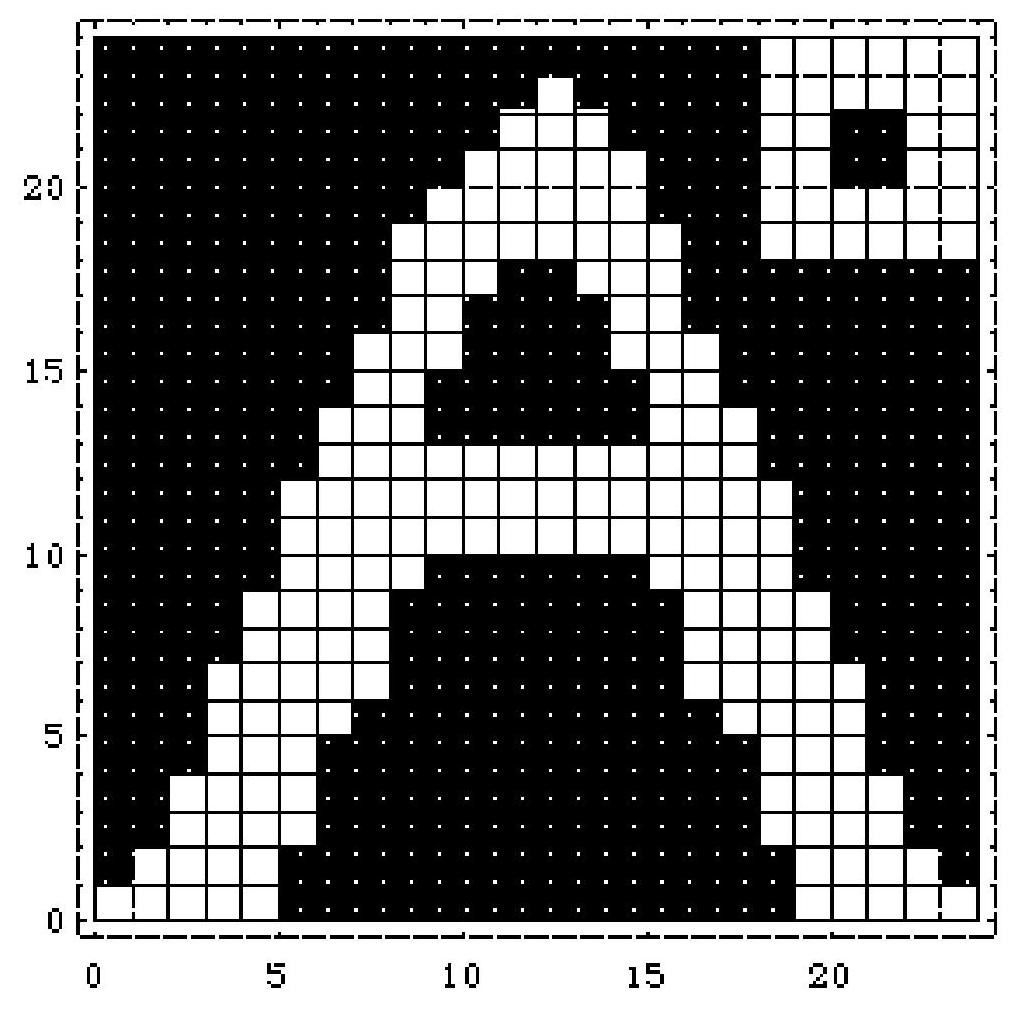
\includegraphics[totalheight=2in]{./fig/6.jpg}
  \caption{$A$ $24 \times 24$ image} 
  \label{fig:6}
\end{figure}

\begin{center}
\begin{tabular}{|llll|}
\hline
$9.5403$ & $6.6288$ & $5.6369$ & $3.4756$ \\
$2.7385$ & $2.2023$ & $1.5835$ & $1.5566$ \\
$1.4207$ & $1.2006$ & $0.9905$ & $0.9258$ \\
$0.7479$ & $0.6744$ & $0.6122$ & $0.4698$ \\
\hline
\end{tabular}
\end{center}

\begin{figure}[htbp]%[htbp]
  \centering
  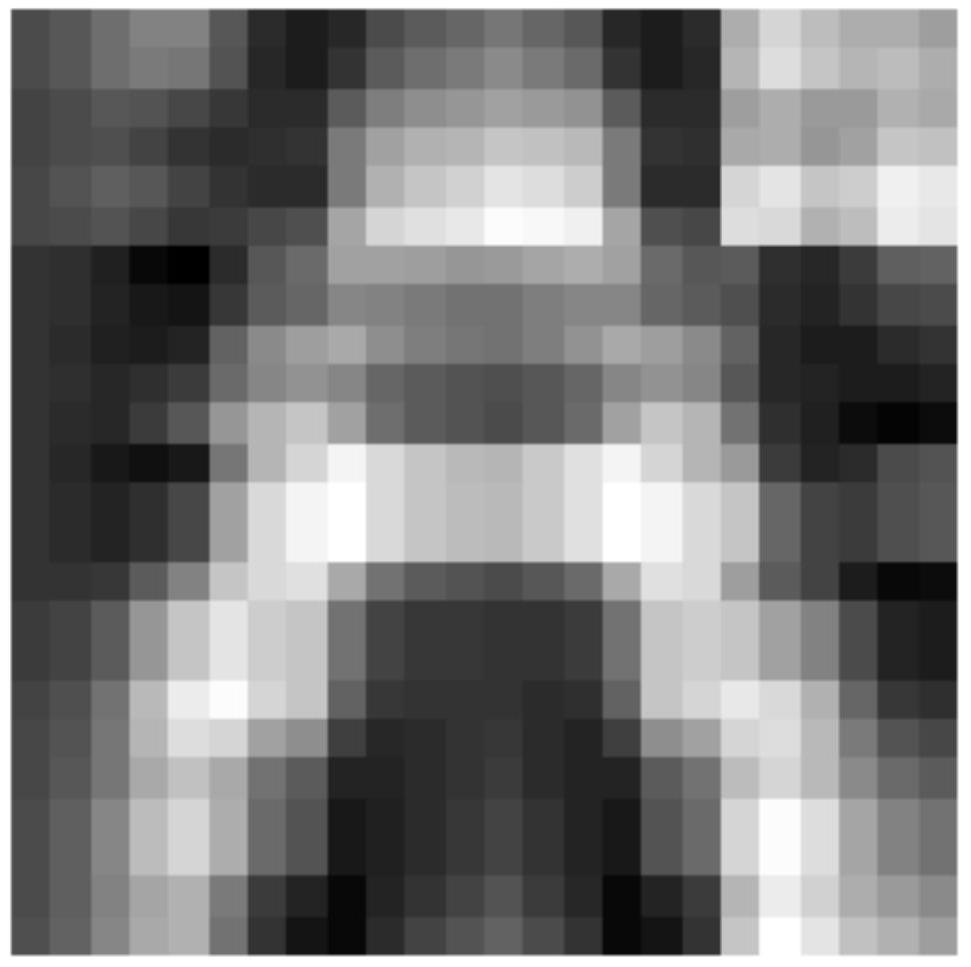
\includegraphics[totalheight=2in]{./fig/7.jpg}
  \caption{秩3近似} 
  \label{fig:7}
\end{figure}

\begin{figure}[htbp]%[htbp]
  \centering
  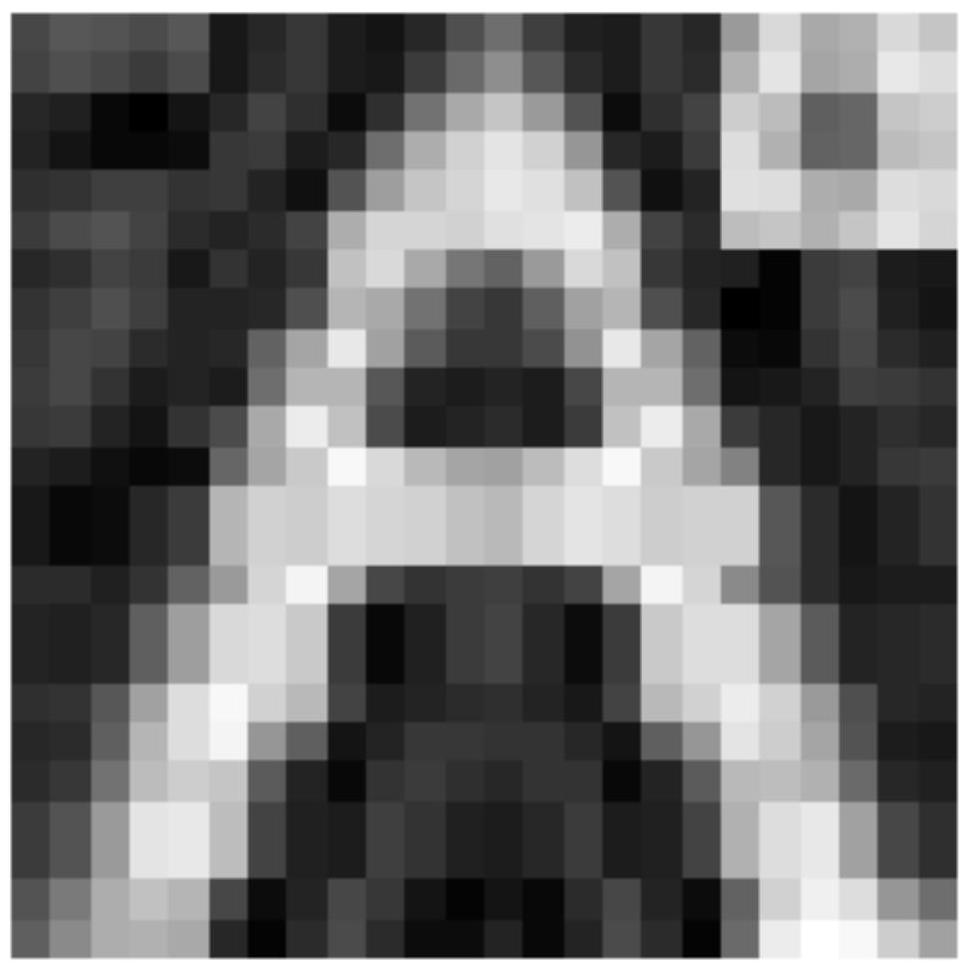
\includegraphics[totalheight=2in]{./fig/8.jpg}
  \caption{秩5近似} 
  \label{fig:8}
\end{figure}

\begin{figure}[htbp]%[htbp]
  \centering
  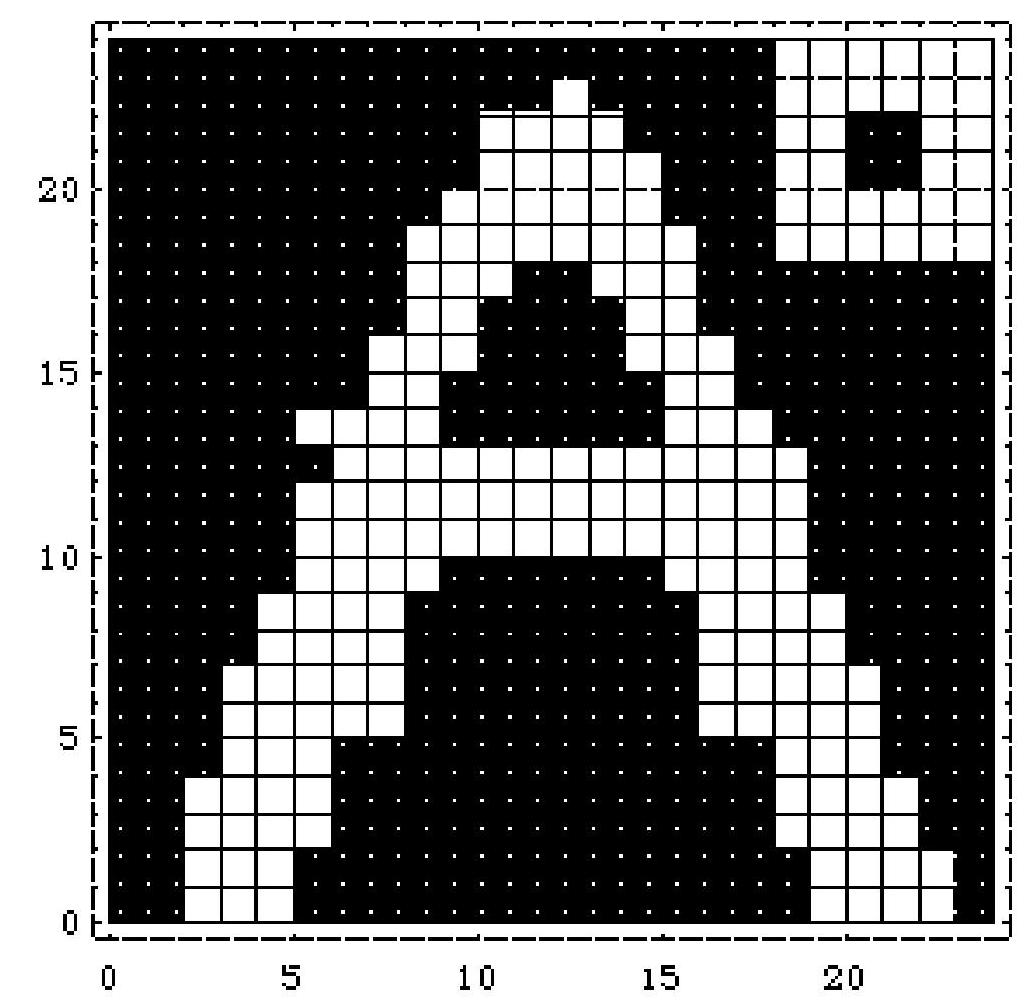
\includegraphics[totalheight=2in]{./fig/9.jpg}
  \caption{秩5近似,四舍五入取整} 
  \label{fig:9}
\end{figure}
现在假设我们采用 $90 \%$ 的准确度阈值。 这意味着我们希望选择误差不超过 $|A|$ 的 $10 \%$ 的降阶近似值。 定义 $e(r)=1-\sqrt{\sum_{1}^{r} \sigma_{i}^{2} / \sum_{1}^{16} \sigma_{i}^{2}} $。 这给出了 SVD 外积扩展的前 $r$ 项之和的相对误差。 计算$e(2)=.18$和$e(3)=.09$,我们看到需要三个展开项才能达到$10\%$或更小的误差。 仅使用系列中的三个项的结果显示为图(\ref{fig:7})中的图像。 这里矩阵的数字条目显示为灰度级。 同样,将阈值设置为 $95 \%$ 将导致我们使用原始矩阵的 5 阶近似值。 这产生了如图(\ref{fig:8})所示的图像,其中可以识别原始图像的主要特征。 事实上,通过简单地将 5 级近似的条目四舍五入到最接近的整数,原始图像几乎可以完美地恢复,如图(\ref{fig:9})所示。 在这方面观察误差矩阵 $E_{5}$ 有 $\left|E_{5}\right|^{2}=\sum_{i>5} \sigma_{i}^{2}=16.7$ . 因此,$E_{5}$ 条目的平方的平均值是 $16.7 / 24^{2}=.029$,我们可以估计条目本身应该在 0.17 左右。 由于该值远低于 0.5,因此图(\ref{fig:9})与原始图像几乎相同也就不足为奇了。

降秩近似和傅里叶分析之间有一个有趣的类比。特别是在离散情况下,傅里叶分析可以被视为表示相对于特殊正交基的数据向量。基本元素被设想为纯振动,即不同频率的正弦和余弦函数。因此,傅里叶分解将输入数据表示为纯振动的叠加,系数指定每个组成频率的幅度。通常,有几个主要频率解释了原始数据中的大部分可变性。剩余的频率可以被丢弃而影响很小。基于 SVD 的降秩近似在意图上非常相似。然而,SVD 为观察到的特定数据捕获了可能的最佳基向量,而不是为所有情况使用一个标准基。出于这个原因,基于 SVD 的降秩近似可以被认为是傅里叶分析的自适应推广。最显着的振动适应出现的特定数据。

\section{SVD 的一种计算算法}
SVD 的适用性是其理论性质的结果。在实际应用中,计算 SVD 的软件被视为一个黑匣子:我们对结果的准确感到满意,并且满足于使用它们而不必担心它们是如何得出的。然而,看看盒子,你会看到一个优雅而强大的想法:隐式矩阵算法。用于计算 $A$ 的 SVD 的标准算法之一背后的基本思想取决于与 $A^{T} A$ 的 EVD 的紧密连接。随着算法的进行,它会生成一系列近似值 $A_{i}=U_{i} \Sigma_{i} V_{i}^{T}$ 到 $A$ 的正确 SVD。 SVD 算法的有效性可以通过证明在每次迭代之后,乘积 $A_{i}^{T} A_{i}$ 正是一个众所周知的算法的相应迭代所产生的$A^{T} A$ 的 EVD。因此,SVD 算法的收敛特性是从 EVD 算法的收敛特性中推断出来的,尽管 $A^{T} A$ 从未计算过且 EVD 算法从未执行过。从这个角度来看,SVD算法可以看作是$A^{T}A$的EVD的隐式算法。它提供了通过直接在 $A$ 上操作来构建 EVD 所需的所有信息。实际上,$A$ 上的操作被视为隐式地执行 $A^{T} A$ 的 EVD 算法,而没有显式地形成 $A^{T} A$。

隐式算法是当前研究兴趣的主题。 参考文献 [1] 和 [4] 描述了除 SVD 之外的一些隐式计算算法,并建议了进一步阅读的来源。 SVD 算法的详细说明见 [8, Sec. 8.3]。 在那里的注释和参考资料中,还给出了一些关于算法历史的附加引文和注释。 在 [7] 中,有一个更紧凑(虽然不太通用)的开发,它使与 $Q R$ 算法的连接更直接。 还应该注意的是,上述算法还有其他选择。 在某些类型的并行处理中具有重要意义的一种替代方法归功于 Jacobi,参见 [8, Sec. 8.4]。 另一个有趣的替代方案使用 rank 1 修改将 SVD 问题拆分为两个较低维度的问题,其结果可用于找到原始问题的 SVD。 这种方法在[11]中有所描述。

\section{结论}
本文的主要目标是使 SVD 引起广大读者的注意。 已经描述了理论性质,并且在第一节线性代数课程中揭示了 SVD 和标准主题之间的密切联系。 提到了 SVD 的几个应用,并详细讨论了两个:最小二乘问题和降秩估计。 还简要提到了 SVD 的计算算法。

在强调主题的主题时,通常有必要省略有趣的细节并将介绍限制在一般性的想法上。 鼓励读者查阅参考资料,以更彻底地处理这种非常有价值的分解的许多方面。

致谢:非常感谢 Bart Braden 编辑对本文做出的重大贡献。 还要感谢 Kevin Kirby 教授在降阶近似示例中使用的数学文件。

\section{References}
[1] Gary E. Adams, Adam W. Bojanzcyk, and Franklin T. Luk, Computing the PSVD of two $2 \times 2$ triangular matrices, SIAM J. Matrix Anal. Appl. vol 15, no 2, pp 366 - 382, April $1994 .$

[2] Harry C. Andrews and Claude L. Patterson, Outer Product Expansions and their uses in digital image processing, The Amer Math Monthly, pp 1-13, January $1975 .$

[3] S. J. Blank, Nishan Krikorian, and David Spring, A geometrically inspired proof of the singular value decomposition, The Amer Math Monthly, pp 238-239, March $1989 .$ [4] Adam Bojanczyk and Paul Van Dooren, On propagating orthogonal transformations in a product of $2 \times 2$ triangular matrices, in Lothar Reichel, Arden Ruttan, and Richard S. Varga, Eds. $N u$ merical Linear Algebra: Proceedings of the Conference in Numerical Linear Algebra and Scientific Computation, Kent (Ohio), March 13-14, 1992, pp 1- 9, W. de Gruyter, New York, $1993 .$

[5] Randall E. Cline, Elements of the theory of generalized inverses for matrices. Education Development Center, Newton, Mass, $1979 .$

[6] K. R. Gabriel, The biplot graphic display of matrices with application to principal components analysis, Biometrika vol 58 , no 3 , pp. $453-467,1971 .$

[7] Gene H. Golub and C. Reinsch, Singular value decomposition and least squares solutions Numer. Math. vol 14, pp. $403-420,1970 .$

[8] Gene H. Golub and Charles F. Van Loan, Matrix Computations, John Hopkins Univ Press, Baltimore, $1983 .$

[9] I. J. Good, Some applications of the singular decomposition of a matrix, Technometrics, vol 11, no $4, \mathrm{pp} 823-831$, Nov $1969 .$

[10] Implicit Matrix Computations. Mini Symposium 36, SIAM 40th anniversary meeting, July 20 - 24, 1992, Los Angeles.

[11] E.R. Jessup and D.C. Sorensen, A Parallel Algorithm for Computing the Singular Value Decomposition of a matrix, SIAM J. Matrix Anal. Appl., vol 15, pp $530-548,1994 .$

[12] David Kahaner, Cleve Moler, and Stephen Nash, Numerical Methods and Software, Prentice Hall, Englewood Cliffs, NJ, $1988 .$

[13] Kevin Kirby, private communication, Northern Kentucky University, Highland Heights, KY $41076 .$

[14] Charles L. Lawson and Richard J. Hanson, Solving Least Squares Problems, Prentice-Hall, Englewood Cliffs, NJ, $1974 .$

[15] David C. Lay, Linear Algebra and its Applications, Addison-Wesley, Reading, MA, $1994 .$

[16] Stephen J. Leon, Linear Algebra with Applications, 4th edition, Macmillan, New York, $1994 .$

[17] Cliff Long, Visualization of matrix singular value decomposition, Mathematics Magazine, vol 56, no 3 , pp161-167, May $1983 .$

[18] The student edition of MATLAB, Prentice Hall, Englewood Cliffs, NJ, $1992 .$

[19] Cleve Moler and Donald Morrison, Singular value analysis of cryptograms, The Amer Math Monthly, pp 78-86, February $1983 .$

[20] Ben Noble and James W. Daniel, Applied Linear Algebra, 2nd edition, Prentice-Hall, Englewood Cliffs, NJ, $1977 .$

[21] John A. Richards, Remote Sensing Digital Image Analysis, Springer-Verlag, New York, $1993 .$ [22] Gilbert Strang, Linear Algebra and its Applications, 2nd edition, Academic Press, New York, $1980 .$

[23] Gilbert Strang, The fundamental theorem of linear algebra, American Mathematical Monthly, Volume 100, number 9 , pp 848 - 859, November $1993 .$
\end{CJK}
\end{document}